\chapter{Descretization of the dynamics}
\label{chap:descretization dynamics}
{\bf \Large 
\begin{tabular}{ccc}
\hline
  Corresponding author & : & Hirofumi Tomita\\
\hline
\end{tabular}
}

\section{Time integration method}

For the time integration of Eqs.(\ref{eq:rhotot_d2})-(\ref{eq:etot_d2}),
we adopt the full explicit scheme with
the $p$-th order Runge-Kutta scheme.
\begin{eqnarray}
&& \phi^{*}_{0} = \phi^{t}\\
&&  \phi^{*}_{1} 
= \phi^{t} + \left(\frac{\partial \phi}{\partial t}\right)^{*}_{0}\frac{\Delta t}{p}\\
&&  \phi^{*}_{2} 
= \phi^{t} + \left(\frac{\partial \phi}{\partial t}\right)^{*}_{1}\frac{\Delta t}{p-1}\\
&&  \cdot \cdot \cdot\nonumber\\
&&  \cdot \cdot \cdot\nonumber\\
&&  \cdot \cdot \cdot\nonumber\\
&&  \phi^{*}_{p} = \phi^{t} + \left(\frac{\partial \phi}{\partial t}\right)^{*}_{p-1} \Delta t\\
&& \phi^{t+\Delta t} = \phi^{*}_{p}
\end{eqnarray}
where $\left(\frac{\partial \phi}{\partial t}\right)^{*}_{k}$ is 
the estimated time tendency by using $\phi^{*}_{k}$.
Usually, we use $p=2,3$ and $4$.

\section{Spatial descretization}
We employ the Arakawa-C staggered grid with the 3-dimensional momentum 
($\rho u, \rho v, \rho w$), density ($\rho$) and mass-weighted potentail temperature($\rho \theta$)
as the prognostic variables.
Figure \ref{fig:cntrl-volume}(a) shows the structure of the control volume for the mass,
indicating the location of each of prognostic variables.
Conceptually, we use the 4th order central difference scheme 
for the advection or convection terms and
the 2nd order central difference scheme for the other terms.
Before the descretization of differential equations,
we should diagnose several quantities from the prognostic variables.
\begin{description}
\item[Full-level pressure and potential temperature]
\begin{eqnarray}
&&p_{i,j,k}=p_{00}\left[\frac{(\rho \theta)_{i,j,k} R^*}{p_{00}} \right]^{\frac{c_{p}^*}{c_{p}^*- R^*}}\\
&&\theta_{i,j,k} = \frac{(\rho \theta)_{i,j,k}}{\rho_{i,j,k}} \label{eq:theta full} \\
\end{eqnarray}
\item[Half-level density]
\begin{eqnarray}
&&  \overline{\rho}_{i+\frac{1}{2},j,k} = \frac{\rho_{i+1,j,k}+\rho_{i,j,k}}{2} \label{eq:rho half i} \\
&&  \overline{\rho}_{i,j+\frac{1}{2},k} = \frac{\rho_{i,j+1,k}+\rho_{i,j,k}}{2} \label{eq:rho half j} \\
&&  \overline{\rho}_{i,j,k+\frac{1}{2}} = \frac{\rho_{i,j,k+1}+\rho_{i,j,k}}{2} \label{eq:rho half k}
\end{eqnarray}
\item[Half-level velocity]
\begin{eqnarray}
&&  \overline{u}_{i+\frac{1}{2},j,k} = \frac{(\rho u)_{i+\frac{1}{2},j,k}}{\overline{\rho}_{i+\frac{1}{2},j,k}}\\
&&  \overline{v}_{i,j+\frac{1}{2},k} = \frac{(\rho v)_{i,j+\frac{1}{2},k}}{\overline{\rho}_{i,j+\frac{1}{2},k}}\\
&&  \overline{w}_{i,j,k+\frac{1}{2}} = \frac{(\rho w)_{i,j,k+\frac{1}{2}}}{\overline{\rho}_{i,j,k+\frac{1}{2}}}
\end{eqnarray}
\item[Full-level velocity]
\begin{eqnarray}
&&  \overline{u}_{i,j,k} = \frac{(\rho u)_{i+\frac{1}{2},j,k}+(\rho u)_{i-\frac{1}{2},j,k}}{2\rho_{i,j,k}} \label{eq:u full} \\
&&  \overline{v}_{i,j,k} = \frac{(\rho v)_{i,j+\frac{1}{2},k}+(\rho v)_{i,j-\frac{1}{2},k}}{2\rho_{i,j,k}} \label{eq:v full} \\
&&  \overline{w}_{i,j,k} = \frac{(\rho w)_{i,j,k+\frac{1}{2}}+(\rho w)_{i,j,k-\frac{1}{2}}}{2\rho_{i,j,k}} \label{eq:w full}
\end{eqnarray}
\end{description}




\subsection{Continuity equation}
\begin{eqnarray}
%%
\left(\frac{\partial \rho}{\partial t}\right)_{i,j,k}
&=& - \frac{(\rho u)_{i+\frac{1}{2},j,k} -(\rho u)_{i-\frac{1}{2},j,k}}{\Delta x}\nonumber\\
& & - \frac{(\rho v)_{i,j+\frac{1}{2},k} -(\rho v)_{i,j-\frac{1}{2},k}}{\Delta y}\nonumber\\
& & - \frac{(\rho w)_{i,j,k+\frac{1}{2}} -(\rho w)_{i,j,k-\frac{1}{2}}}{\Delta z}
\end{eqnarray}

\subsection{Momentum equations}
Figure \ref{fig:cntrl-volume}(a) shows the structure of the control volume for the momentum
in the x direction.
The momentum equation is descretized as
\begin{eqnarray}
%%
\left(\frac{\partial \rho u}{\partial t}\right)_{i+\frac{1}{2},j,k}
&=& - \frac{\overline{(\rho u)}_{i+1,j,k} \overline{u}_{i+1,j,k} 
           -\overline{(\rho u)}_{i,j,k} \overline{u}_{i,j,k}}
     {\Delta x}\nonumber\\
& & - \frac{\overline{(\rho u)}_{i+\frac{1}{2},j+\frac{1}{2},k}  \overline{v}_{i+\frac{1}{2},j+\frac{1}{2},k} 
           -\overline{(\rho u)}_{i+\frac{1}{2},j-\frac{1}{2},k}  \overline{v}_{i+\frac{1}{2},j-\frac{1}{2},k}}
     {\Delta y}\nonumber\\
& & - \frac{\overline{(\rho u)}_{i+\frac{1}{2},j,k+\frac{1}{2}}  \overline{w}_{i+\frac{1}{2},j,k+\frac{1}{2}} 
           -\overline{(\rho u)}_{i+\frac{1}{2},j,k-\frac{1}{2}}  \overline{w}_{i+\frac{1}{2},j,k-\frac{1}{2}}}
     {\Delta z}\nonumber\\
& & -\frac{p_{i+1,j,k}-p_{i,j,k}}{\Delta x},
\end{eqnarray}
where 
\begin{eqnarray}
&& \overline{(\rho u)}_{i,j,k} \nonumber\\
= && \frac{-(\rho u)_{i+\frac{3}{2},j,k}+7(\rho u)_{i+\frac{1}{2},j,k}+7(\rho u)_{i-\frac{1}{2},j,k}-(\rho u)_{i-\frac{3}{2},j,k}}{12}\\
&& \overline{(\rho u)}_{i+\frac{1}{2},j+\frac{1}{2},k} \nonumber\\
= && \frac{-(\rho u)_{i+\frac{1}{2},j+2,k}+7(\rho u)_{i+\frac{1}{2},j+1,k}+7(\rho u)_{i+\frac{1}{2},j,k}-(\rho u)_{i+\frac{1}{2},j-1,k}}{12}\\
&& \overline{(\rho u)}_{i+\frac{1}{2},j,k+\frac{1}{2}} \nonumber\\
= &&\frac{-(\rho u)_{i+\frac{1}{2},j,k+2}+7(\rho u)_{i+\frac{1}{2},j,k+1}+7(\rho u)_{i+\frac{1}{2},j,k}-(\rho u)_{i+\frac{1}{2},j,k-1}}{12}
\end{eqnarray}
and the velocities at the cell wall for the staggered control volume to $x$ direction are
defined as
\begin{eqnarray}
\overline{u}_{i,j,k} &=& \frac{\overline{u}_{i+\frac{1}{2},j,k}+\overline{u}_{i-\frac{1}{2},j,k}}{2}\\
\overline{v}_{i+\frac{1}{2},j+\frac{1}{2},k} &=& 
\frac{\overline{v}_{i,j+\frac{1}{2},k}+\overline{v}_{i+1,j+\frac{1}{2},k}}{2}\\
\overline{w}_{i+\frac{1}{2},j,k+\frac{1}{2}} &=& 
\frac{\overline{w}_{i,j,k+\frac{1}{2}}+\overline{w}_{i+1,j,k+\frac{1}{2}}}{2}
\end{eqnarray}
In this form, the 4th order accuracy is guaranteed 
on the condition of the constant velocity.

The momentum equations in the $y$ and $z$ directions are descretized 
in the same way:
\begin{eqnarray}
%%
\left(\frac{\partial \rho v}{\partial t}\right)_{i,j+\frac{1}{2},k}
&=& - \frac{\overline{(\rho v)}_{i+\frac{1}{2},j+\frac{1}{2},k}  \overline{u}_{i+\frac{1}{2},j+\frac{1}{2},k} 
           -\overline{(\rho v)}_{i-\frac{1}{2},j+\frac{1}{2},k}  \overline{u}_{i-\frac{1}{2},j+\frac{1}{2},k}}
     {\Delta x}\nonumber\\
& & - \frac{\overline{(\rho v)}_{i,j+1,k} \overline{v}_{i,j+1,k} 
           -\overline{(\rho v)}_{i,j,k} \overline{v}_{i,j,k}}
     {\Delta y}\nonumber\\
& & - \frac{\overline{(\rho v)}_{i,j+\frac{1}{2},k+\frac{1}{2}}  \overline{v}_{i,j+\frac{1}{2},k+\frac{1}{2}} 
           -\overline{(\rho v)}_{i,j+\frac{1}{2},k-\frac{1}{2}}  \overline{v}_{i,j+\frac{1}{2},k-\frac{1}{2}}}
     {\Delta z}\nonumber\\
& & -\frac{p_{i,j+1,k}-p_{i,j,k}}{\Delta y},\\
%%
\left(\frac{\partial \rho w}{\partial t}\right)_{i,j,k+\frac{1}{2}}
&=& - \frac{\overline{(\rho w)}_{i+\frac{1}{2},j,k+\frac{1}{2}}  \overline{u}_{i+\frac{1}{2},j,k+\frac{1}{2}} 
           -\overline{(\rho w)}_{i-\frac{1}{2},j,k+\frac{1}{2}}  \overline{u}_{i-\frac{1}{2},j,k+\frac{1}{2}}}
     {\Delta x}\nonumber\\
& & - \frac{\overline{(\rho w)}_{i,j+\frac{1}{2},k+\frac{1}{2}}  \overline{w}_{i,j+\frac{1}{2},k+\frac{1}{2}} 
           -\overline{(\rho w)}_{i,j-\frac{1}{2},k+\frac{1}{2}}  \overline{w}_{i,j-\frac{1}{2},k+\frac{1}{2}}}
     {\Delta y}\nonumber\\
& & - \frac{\overline{(\rho w)}_{i,j,k+1} \overline{w}_{i,j,k+1} 
           -\overline{(\rho w)}_{i,j,k} \overline{w}_{i,j,k}}
     {\Delta z}\nonumber\\
& & -\frac{p_{i,j,k+1}-p_{i,j,k}}{\Delta z}-\overline{\rho}_{i,j,k+\frac{1}{2}} g
\end{eqnarray}

\subsection{Energy equation}

\begin{eqnarray}
%%
\left(\frac{\partial \rho \theta}{\partial t}\right)_{i,j,k}
&=& - \frac{(\rho u)_{i+\frac{1}{2},j,k} \overline{\theta}_{i+\frac{1}{2},j,k} 
           -(\rho u)_{i-\frac{1}{2},j,k} \overline{\theta}_{i-\frac{1}{2},j,k}}
     {\Delta x}\nonumber\\
& &  - \frac{(\rho v)_{i,j+\frac{1}{2},k} \overline{\theta}_{i,j+\frac{1}{2},k} 
           -(\rho v)_{i,j-\frac{1}{2},k} \overline{\theta}_{i,j-\frac{1}{2},k}}
     {\Delta y}\nonumber\\
& &  - \frac{(\rho w)_{i,j,k+\frac{1}{2}} \overline{\theta}_{i,j,k+\frac{1}{2}} 
           -(\rho w)_{i,j,k-\frac{1}{2}} \overline{\theta}_{i,j,k-\frac{1}{2}}}
     {\Delta z}\nonumber\\
\end{eqnarray}
where
\begin{eqnarray}
&& \overline{\theta}_{i+\frac{1}{2},j,k} = 
\frac{-\theta_{i+2,j,k}+7\theta_{i+1,j,k}+7\theta_{i,j,k}-\theta_{i-1,j,k}}{12}\\
&& \overline{\theta}_{i,j+\frac{1}{2},k} = 
\frac{-\theta_{i,j+2,k}+7\theta_{i,j+1,k}+7\theta_{i,j,k}-\theta_{i,j-1,k}}{12}\\
&& \overline{\theta}_{i,j,k+\frac{1}{2}} = 
\frac{-\theta_{i,j,k+2}+7\theta_{i,j,k+1}+7\theta_{i,j,k}-\theta_{i,j,k-1}}{12}
\end{eqnarray}

\subsection{Tracer advection}
The tracer advection process is done after the time integration of 
the dynamical variables ($\rho$, $\rho u,\rho v,\rho w$, and $\rho \theta$).
We impose two constraints to tracer advection:
\begin{description}
\item[Consistency With Continuity ( CWC )]
On the condition without any source/sink,
the mass concentration in the advection process 
should be conserved along the trajectory.
It is, at least,  necessary that 
the spatially constant mass concentration should be kept
in any motion of fluid.
In order to satisfy this condition, we use the same mass flux at the last Runge-Kutta
process of Eqs.() and () for integration of tracers:
\begin{eqnarray}
%%
\frac{\left(\rho q\right)^{n+1}_{i,j,k} - \left(\rho q\right)^{n}_{i,j,k}}{\Delta t}
&=& - \frac{(\rho u)_{i+\frac{1}{2},j,k} \overline{q}_{i+\frac{1}{2},j,k} 
           -(\rho u)_{i-\frac{1}{2},j,k} \overline{q}_{i-\frac{1}{2},j,k}}
     {\Delta x}\nonumber\\
& &  - \frac{(\rho v)_{i,j+\frac{1}{2},k} \overline{q}_{i,j+\frac{1}{2},k} 
           -(\rho v)_{i,j-\frac{1}{2},k} \overline{q}_{i,j-\frac{1}{2},k}}
     {\Delta y}\nonumber\\
& &  - \frac{(\rho w)_{i,j,k+\frac{1}{2}} \overline{q}_{i,j,k+\frac{1}{2}} 
           -(\rho w)_{i,j,k-\frac{1}{2}} \overline{q}_{i,j,k-\frac{1}{2}}}
     {\Delta z}\nonumber\\
\label{eq:tracer_int}
\end{eqnarray}
\item[Monotonicity]
In order to satisfy the monotonicity of tracer advection,
we employ the Flux Corrected Trasport scheme, which is a hybrid scheme 
with the 4th order central difference scheme and 1st order upwind scheme.
If The 4th order central difference is applied, 
$\overline{q}$ is descritized as
\begin{eqnarray}
&& \overline{q}_{i+\frac{1}{2},j,k}^{high} = 
\frac{-q_{i+2,j,k}+7q_{i+1,j,k}+7q_{i,j,k}-q_{i-1,j,k}}{12}\\
&& \overline{q}_{i,j+\frac{1}{2},k}^{high} = 
\frac{-q_{i,j+2,k}+7q_{i,j+1,k}+7q_{i,j,k}-q_{i,j-1,k}}{12}\\
&& \overline{q}_{i,j,k+\frac{1}{2}}^{high} = 
\frac{-q_{i,j,k+2}+7q_{i,j,k+1}+7q_{i,j,k}-q_{i,j,k-1}}{12}.
\end{eqnarray}
On the other hand, in the 1st order upwind scheme 
$\overline{q}$ is described as
\begin{eqnarray}
\overline{q}_{i+\frac{1}{2},j,k}^{low} = 
\begin{cases}
  q_{i,j,k} & ( (\rho u)_{i+\frac{1}{2},j,k}>0 )\\
  q_{i+1,j,k} & ({\rm otherwise})\\
\end{cases}
\\
\overline{q}_{i,j+\frac{1}{2},k}^{low} = 
\begin{cases}
  q_{i,j,k} & ( (\rho u)_{i,j+\frac{1}{2},k}>0 )\\
  q_{i,j+1,k} & ({\rm otherwise})\\
\end{cases}
\\
\overline{q}_{i,j,k+\frac{1}{2}}^{low} = 
\begin{cases}
  q_{i,j,k} & ( (\rho u)_{i,j,k+\frac{1}{2}}>0 )\\
  q_{i,j,k+1} & ({\rm otherwise})\\
\end{cases}
\end{eqnarray}
The actual $\overline{q}$ is described as
\begin{eqnarray}
  \overline{q}_{i+\frac{1}{2},j,k}  
&=& C_{i+\frac{1}{2},j,k} \overline{q}_{i+\frac{1}{2},j,k}^{high}
+ \left( 1 - C_{i+\frac{1}{2},j,k}\right) \overline{q}_{i+\frac{1}{2},j,k}^{low}\\
  \overline{q}_{i,j+\frac{1}{2},k}  
&=& C_{i,j+\frac{1}{2},k} \overline{q}_{i,j+\frac{1}{2},k}^{high}
+ \left( 1 - C_{i,j+\frac{1}{2},k}\right) \overline{q}_{i,j+\frac{1}{2},k}^{low}\\
  \overline{q}_{i,j,k+\frac{1}{2}}  
&=& C_{i,j,k+\frac{1}{2}} \overline{q}_{i,j,k+\frac{1}{2}}^{high}
+ \left( 1 - C_{i,j,k+\frac{1}{2}}\right) \overline{q}_{i,j,k+\frac{1}{2}}^{low}
\end{eqnarray}
See the appedix for the method to determine the flux limter.
\end{description}



\section{boundary condition}
The boundary condition only for the vertical velocity at the top and bottom
boundaries is needed:
\begin{eqnarray}
&&  w_{i,j,k_{max}+\frac{1}{2}} = 0\\
&&  w_{i,j,k_{min}-\frac{1}{2}} = 0
\end{eqnarray}
This leads to the boundary condition of the prognostic variable as
\begin{eqnarray}
&&  (\rho w)_{i,j,k_{max}+\frac{1}{2}} = 0\\
&&  (\rho w)_{i,j,k_{min}-\frac{1}{2}} = 0
\end{eqnarray}



\section{Numerical filters}

In the dynamics exept for the tracer advection,
we can consider two ways to stabilize the calculation conceptually.
\begin{enumerate}
\item We impose no explicit numerical filter.
The numerical stability can be achieved
by aid of tiny portion of turbulence scheme.
\item We impose tiny explicit numerical filter by the numerical viscousity or diffusion.
In order to damp the higher wavenumber component selectively,
we adapt the super-viscousty or diffusion as the traditional way.
\end{enumerate}
In this section, we formulate the latter case.
The Laplacian of an arbitray prognostic valuable $f (\in \rho, u, v, w, \theta)$ 
is descritized as
{\footnotesize
\begin{eqnarray}
(\Delta f)_i &=& 
\frac{1}{\Delta x_i}\left[
\frac{1}{\Delta x_{i+\frac{1}{2}}}f_{i+1}
-\left(\frac{1}{\Delta x_{i+\frac{1}{2}}}+\frac{1}{\Delta x_{i-\frac{1}{2}}}\right)f_i
+\frac{1}{\Delta x_{i-\frac{1}{2}}}f_{i-1}\right]
%
\end{eqnarray}
}
The super-diffusion can be descritezed as
{\footnotesize
\begin{eqnarray}
&&\frac{\partial }{\partial x}\left[\nu \rho \frac{\partial \Delta f}{\partial x}\right]  =\nonumber\\
&&
\frac{1}{\Delta x_{i}}
\Bigg[\nonumber\\
&&\frac{\nu_{i+\frac{1}{2}}\rho_{i+\frac{1}{2}}}{\Delta x_{i+\frac{1}{2}}}
\Bigg\{\frac{1}{\Delta x_{i+1}}\left[
\frac{1}{\Delta x_{i+\frac{3}{2}}}f_{i+2}
-\left(\frac{1}{\Delta x_{i+\frac{3}{2}}}+\frac{1}{\Delta x_{i+\frac{1}{2}}}\right)f_{i+1}
+\frac{1}{\Delta x_{i+\frac{1}{2}}}f_{i}\right]\nonumber\\
&&~~~~~~~~~~~~ -\frac{1}{\Delta x_i}\left[
\frac{1}{\Delta x_{i+\frac{1}{2}}}f_{i+1}
-\left(\frac{1}{\Delta x_{i+\frac{1}{2}}}+\frac{1}{\Delta x_{i-\frac{1}{2}}}\right)f_i
+\frac{1}{\Delta x_{i-\frac{1}{2}}}f_{i-1}\right]\Bigg\}
\nonumber\\
%
&-&
\frac{\nu_{i-\frac{1}{2}}\rho_{i-\frac{1}{2}}}{\Delta x_{i-\frac{1}{2}}}
\Bigg\{\frac{1}{\Delta x_{i}}\left[
\frac{1}{\Delta x_{i+\frac{1}{2}}}f_{i+1}
-\left(\frac{1}{\Delta x_{i+\frac{1}{2}}}+\frac{1}{\Delta x_{i-\frac{1}{2}}}\right)f_{i}
+\frac{1}{\Delta x_{i-\frac{1}{2}}}f_{i-1}\right]\nonumber\\
&&~~~~~~~~~~~~ -\frac{1}{\Delta x_{i-1}}\left[
\frac{1}{\Delta x_{i-\frac{1}{2}}}f_{i}
-\left(\frac{1}{\Delta x_{i-\frac{1}{2}}}+\frac{1}{\Delta x_{i-\frac{3}{2}}}\right)f_{i-1}
+\frac{1}{\Delta x_{i-\frac{3}{2}}}f_{i-2}\right]\Bigg\}\nonumber\\
&&\Bigg]
%
%
\end{eqnarray}
}
In Eq.(), the numerical diffiusion flux can be written as
{\footnotesize
\begin{eqnarray}
F_{i+\frac{1}{2}}&=&\frac{\nu_{i+\frac{1}{2}}\rho_{i+\frac{1}{2}}}{\Delta x_{i+\frac{1}{2}}}
\Bigg\{\frac{1}{\Delta x_{i+1}}\left[
\frac{1}{\Delta x_{i+\frac{3}{2}}}f_{i+2}
-\left(\frac{1}{\Delta x_{i+\frac{3}{2}}}+\frac{1}{\Delta x_{i+\frac{1}{2}}}\right)f_{i+1}
+\frac{1}{\Delta x_{i+\frac{1}{2}}}f_{i}\right]\nonumber\\
&&~~~~~~~~~~~~ -\frac{1}{\Delta x_i}\left[
\frac{1}{\Delta x_{i+\frac{1}{2}}}f_{i+1}
-\left(\frac{1}{\Delta x_{i+\frac{1}{2}}}+\frac{1}{\Delta x_{i-\frac{1}{2}}}\right)f_i
+\frac{1}{\Delta x_{i-\frac{1}{2}}}f_{i-1}\right]\Bigg\}\nonumber\\
\end{eqnarray}
}
The coefficient $\nu$ is determined by
\begin{eqnarray}
  \nu_{i+\frac{1}{2}} &=& \gamma \frac{\Delta x_{i+\frac{1}{2}}^4}{\Delta t}
\end{eqnarray}
where  the $\gamma$ is non-dimensional coefficient and it should satisfy that
\begin{eqnarray}
\gamma < \frac{1}{16}
\end{eqnarray}
for the numerical stability of numerical filter itself.
If Eq.() is rewritten by using Eq.(), 
\begin{eqnarray}
\frac{\partial }{\partial x}\left[\nu \rho \frac{\partial \Delta f}{\partial x}\right]  
=
\frac{F_{i+\frac{1}{2}}-F_{i-\frac{1}{2}}}{\Delta x_{i}}
%
%
\end{eqnarray}
In this numerical diffusion process,
we can consider that the advective flux is modified as
\begin{eqnarray}
  (\rho u f)_{i+\frac{1}{2}}^{\dagger} = (\rho u f)_{i+\frac{1}{2}}+F_{i+\frac{1}{2}}
\end{eqnarray}
where the first term of R.H.S. is the flux by the advection scheme.
In this dynamics, it is the 4th order central difference scheme.
This concept is very important for the CWC condition in the continuity equation.
The mass flux in the tracer advection should be used as this formulation, 
otherwize the CWC condition is violated.

The numerical diffusion in the $y$ and $z$ directions
are formulated in the same way.



\begin{figure}[t]
\begin{center}
  \begin{tabular}{l}
    (a) Control volume for the mass\\
  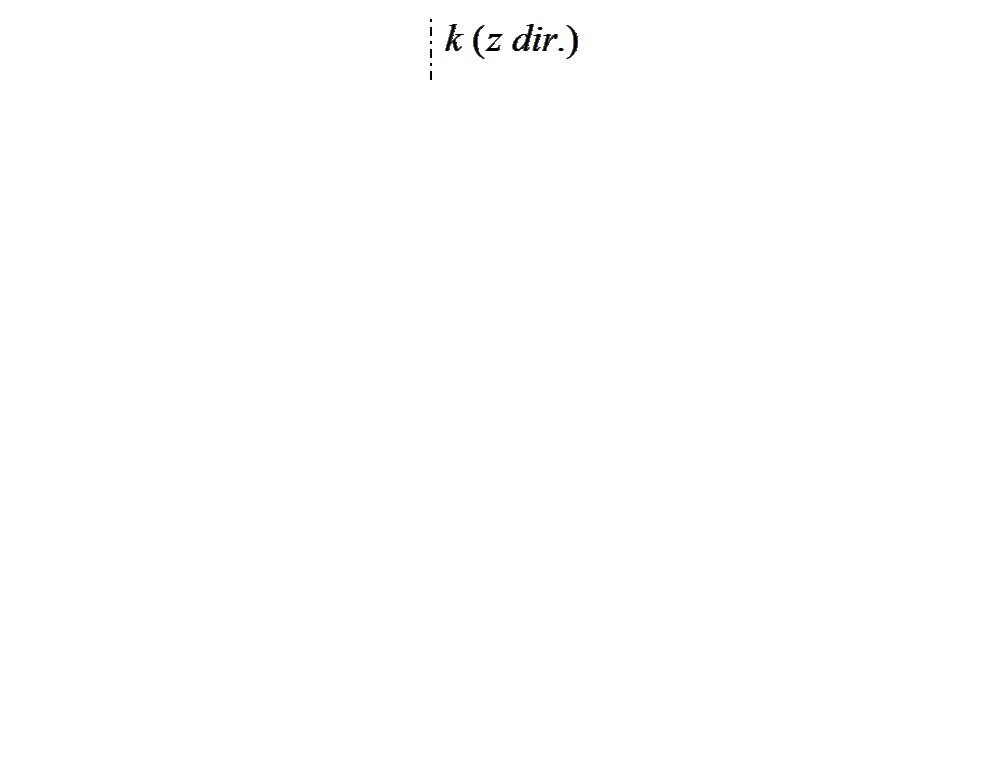
\includegraphics[scale=0.6]{./figure/cntrl-volume.eps}\\
    (b) Control volume for the momentum\\
  \includegraphics[scale=0.6]{./figure/cntrl-volume2.eps}\\
  \end{tabular}
\end{center}
  \caption{Control volume}
  \label{fig:cntrl-volume}
\end{figure}
